\documentclass[11pt,a4paper]{article}

% ---------------------------------------------------------------------------
% Exact common-activity compatibility for autocatalytic junction--path
% assemblies: boundary reduction, a rational decision algorithm, and
% operating certificates.
%
% Author metadata: fill in the three macros below before submission.
% ---------------------------------------------------------------------------
\newcommand{\PaperAuthor}{}
\newcommand{\PaperAffiliation}{}
\newcommand{\PaperDate}{14 September 2026}

\usepackage[T1]{fontenc}
\usepackage[utf8]{inputenc}
\usepackage{lmodern}
\usepackage{microtype}
\usepackage[a4paper,margin=1.05in]{geometry}
\usepackage{amsmath,amssymb,amsthm,mathtools}
\usepackage{booktabs}
\usepackage{array}
\usepackage{enumitem}
\usepackage{xcolor}
\usepackage{graphicx}
\usepackage{tikz}
\usetikzlibrary{arrows.meta,positioning,calc}
\usepackage[obeyspaces,spaces]{url}
\usepackage[numbers,sort&compress]{natbib}
\usepackage[colorlinks=true,linkcolor=blue!55!black,citecolor=blue!55!black,urlcolor=blue!55!black]{hyperref}
\hypersetup{pdftitle={Exact common-activity compatibility for autocatalytic junction-path assemblies},
  pdfsubject={Boundary reduction, rational decision algorithm, and operating certificates for weighted two-reaction autocatalytic cores}}

\DeclareUrlCommand\lean{\urlstyle{tt}}
\setlist{itemsep=2pt,topsep=3pt}
\setlength{\emergencystretch}{1.5em}

\theoremstyle{plain}
\newtheorem{theorem}{Theorem}[section]
\newtheorem{proposition}[theorem]{Proposition}
\newtheorem{lemma}[theorem]{Lemma}
\newtheorem{corollary}[theorem]{Corollary}
\theoremstyle{definition}
\newtheorem{definition}[theorem]{Definition}
\newtheorem{example}[theorem]{Example}
\theoremstyle{remark}
\newtheorem{remark}[theorem]{Remark}
\newtheorem{question}[theorem]{Question}

\newcommand{\R}{\mathbb{R}}
\newcommand{\Q}{\mathbb{Q}}
\newcommand{\Z}{\mathbb{Z}}
\newcommand{\N}{\mathbb{N}}
\newcommand{\rev}{\rightleftharpoons}
\newcommand{\ru}{r_{e,u}}
\newcommand{\rv}{r_{e,v}}
\newcommand{\Abound}{\mathcal{A}}
\newcommand{\src}{\operatorname{src}}
\newcommand{\dst}{\operatorname{dst}}
\newcommand{\Lip}{\operatorname{Lip}}

\title{Exact common-activity compatibility for autocatalytic junction--path assemblies:\\ boundary reduction, a rational decision algorithm, and operating certificates}
\author{\PaperAuthor\\ \PaperAffiliation}
\date{\PaperDate}

\begin{document}
\maketitle

\begin{abstract}
Autocatalytic cores that are each realizable in isolation need not be realizable together: under thermodynamically consistent mass action, every reaction that involves a species sees the same activity of that species, and the stoichiometric powers of the activities constrain both the direction and the magnitude of every current. Kosc, Kuperberg, Rajon and Charlat (\emph{Proc.\ Natl.\ Acad.\ Sci.\ USA}, 2025) proved that every isolated potential autocatalytic core admits a productive realization and exhibited two cores with no common one. We study a class of assemblies in which the number of species is unbounded and compatibility is nevertheless decided exactly. An assembly consists of weighted two-reaction cores $X_u\rev X_v$, $X_v+F\rev 2X_u$ with arbitrary positive kinetic factors, arranged in directed paths whose interiors are private and whose endpoints belong to a set of $k$ shared junction species, each species carrying a closed activity box. We prove that a common activity vector making every selected core strictly productive exists if and only if the junction activities alone satisfy, for each path, a strict inequality between two explicitly composed quadratic responses, together with the junction boxes. The interior of every path is eliminated without relaxing a single current law, and a one-parameter interpolation reconstructs it. For rational data this yields a complete decision procedure that also outputs a rational common state; its total bit cost and output length are at most $\Abound^{O(k+1)}$ with $\Abound=(n+M+k+2)(2^h+1)(B+h+1)$, where $n$ is the input size, $M$ the number of paths, $h$ their maximum length and $B$ the rational height of the data. The precision analysis, which combines a reciprocal root bound for a one-block quantifier-elimination output with Lipschitz control of the composed responses, replaces algebraic sample points by dyadic bisection and handles singleton junction boxes. We further give a linear-programming sufficient certificate that produces explicit compatible assemblies without any integer grading, a sharp fixed-state tolerance radius for independent relative factor uncertainty, an eight-corner certificate for joint activity, factor and food uncertainty, exact food-activity windows, and instantaneous loss budgets. The source-level equivalence, the path reconstruction, the merge across shared species, the rational certificate checker and every local certificate lemma are verified in Lean~4 against Mathlib with warnings promoted to errors and no admitted statements; the quantifier-elimination instantiation, the bit-size accounting and the linear-programming complexity are conventional proofs and are marked as such.
\end{abstract}

\section{Introduction}\label{sec:intro}

A \emph{potential autocatalytic core} (PAC) is a minimal motif of a reaction network that admits a strictly productive reaction current \citep{blokhuis2020,kosc2025}. Whether such a current can be realized by an actual concentration vector is a separate question. Under mass action with fixed transition-state factors the current of a reversible reaction is a positive multiple of the difference of its reactant and product complex activities, and a complex activity is a monomial in the species activities. Kosc, Kuperberg, Rajon and Charlat proved that every isolated PAC is realizable in this sense and showed that two cores sharing a species may admit a common productive current but no common concentration vector \citep{kosc2025}. Two predecessor papers quantified this phenomenon: an exact phase diagram for a pair of overlapping triangles and a layered account of the failure mechanisms \citep{tcic2026}, and, for families of two-reaction cores, minimally incompatible families of every order, an exact univariate elimination for bounded fans, and a polynomial-time constructive certificate for \emph{graded} assemblies, in which integer ranks increase by one along every core \citep{tcch2026}. The graded certificate is sufficient only, the fan theorem fixes a single shared reaction, and the unbounded-order theorem shows that no test based on bounded subfamilies can decide compatibility in general.

This paper isolates a class of assemblies that sits between those results: the number of species and of cores is unbounded, the kinetic factors are arbitrary positive reals that differ from core to core, integer grading is not assumed, and yet compatibility is decided exactly with a rational witness. The class consists of \emph{junction--path assemblies}: the selected cores are partitioned into directed paths whose interior species are private to one path and whose endpoints belong to a designated set of $k$ junction species (Figure~\ref{fig:topology}). Junctions may carry any number of paths and form an arbitrary skeleton. Each species carries a closed activity box; junction boxes may be singletons.

\paragraph{Main results.} Write each selected core $e\colon u\to v$ as $X_u\rev X_v$, $X_v+F\rev 2X_u$ with positive factors $a_e,b_e$ and food activity one, so that its two currents are $p_e=a_e(x_u-x_v)$ and $q_e=b_e(x_v-x_u^2)$, and call it productive when both of its internal species are net produced, $2q_e-p_e>0$ and $p_e-q_e>0$.
\begin{enumerate}[label=(\Alph*)]
\item \emph{Boundary reduction} (Theorems~\ref{thm:path} and~\ref{thm:main}). A single core is productive exactly when $G_e(x_u)<x_v<F_e(x_u)$ for two explicit quadratic responses. Along a path the responses compose in physical order, and every endpoint value strictly between the composed responses is attained by a productive interior whose values stay between the endpoints. Consequently a common productive state in the prescribed boxes exists if and only if the $k$ junction activities satisfy the composed strict inequalities and their boxes. No current law is relaxed, and no species receives two activities.
\item \emph{Exact rational algorithm} (Theorem~\ref{thm:algorithm}). For rational factors and boxes the reduced system is decided by one block of $k$ existentially quantified variables, and a rational common state is reconstructed by dyadic bisection with a proved precision bound. The total bit cost and output length are at most $\Abound^{O(k+1)}$ with $\Abound=(n+M+k+2)(2^h+1)(B+h+1)$. For fixed $k$ and $h=O(\log n)$ this is polynomial in the binary input size.
\item \emph{A linear sufficient class} (Proposition~\ref{prop:linear}). Near the equilibrium point $x\equiv1$ the exact residual identities reduce to a homogeneous strict linear system in \emph{deficits}, decided by a rational linear program. This produces compatible assemblies that admit no integer grading, for instance a nine-species unit-factor assembly of two private paths of lengths four and five.
\item \emph{Operating certificates} (Section~\ref{sec:operating}). At a fixed productive state we give the sharp radius $\rho_*$ of independent relative factor uncertainty, an eight-corner certificate for joint activity, factor and food rectangles, the exact food-activity window, and instantaneous loss budgets, all as closed rational formulas.
\end{enumerate}
Theorem~\ref{thm:main} is a statement about \emph{existence} for arbitrary positive real factors; rationality and the parameters $k,h$ enter only in the algorithm. The obstruction examples of \citep{tcch2026} sit inside the class: a directed cycle is never compatible, and the unit-factor path with a shortcut is never compatible, whereas the same shortcut graph with factors $(9,1),(9,1),(2,1)$ has an explicit rational common state (Section~\ref{sec:operating}). Kinetic factors therefore change the answer without changing the PAC status or the architecture of the cores.

\paragraph{Method.} The one-edge inequality is a rearrangement of the literal currents. Its composition along a path uses only that both responses are strictly increasing on $[0,1]$ and fix $0$ and $1$. Sufficiency is the substantive step: we interpolate between the lower and upper response of every edge with one common parameter $\lambda$ and apply the intermediate value theorem to the endpoint. This constructs a productive interior with the prescribed final activity exactly, which is what allows the interior to be discarded and later rebuilt with rational values. The algorithmic part rests on a published one-block quantifier-elimination bound \citep[Theorem 2.27]{basu2014}, \citep{bpr2006}, used in two roles: as the decision routine, and, with one free slack variable, as a way to bound the size of a positive residual that some feasible point must have. A reciprocal Cauchy bound on the coefficients of the eliminated univariate formula gives a dyadic slack in $H+3$ trials; the composed responses are $2^h$-Lipschitz, which turns that slack into a bracket width; bisection of closed brackets keeps a common real witness and finally yields rational midpoints whose residuals stay positive. Private values are recovered by bisection in the interpolation parameter with an explicit last-edge margin, without root isolation or a number-field compositum.

\paragraph{What is verified.} The chemical equivalence of Theorem~\ref{thm:main} is a Lean~4 theorem stated on the literal reversible network with activity monomials and global species identities, and the rational state checker, the examples and all local certificate lemmas of Sections~\ref{sec:linear} and~\ref{sec:operating} are compiled in the same development \citep{demoura2021,mathlib2020}. Theorem~\ref{thm:algorithm} and the linear-programming complexity are conventional proofs building on cited algorithms. Section~\ref{sec:formal} lists the boundary precisely.

\paragraph{What is not claimed.} We decide compatibility for a supplied decomposition; we do not find an optimal one. Private species share a common box $[\ell,1]$; arbitrary independent private boxes are outside the theorem, and Remark~\ref{rem:privatebox} shows why. The results are static: they concern the existence of one activity vector at which every selected core is productive, not persistence, steady states or long-time behaviour of a dynamical system. The complexity bound is not a fixed-parameter-tractability result in $k$ and the exponential degree $2^h$ of the expanded responses is a property of one representation, not a lower bound.

\paragraph{Organization.} Section~\ref{sec:model} fixes the network, the cores and the class. Section~\ref{sec:edge} proves the one-edge interval and its regularity, Section~\ref{sec:path} the path reconstruction, and Section~\ref{sec:assembly} the assembly theorem. Section~\ref{sec:algorithm} gives the rational algorithm and its bit bound, with a small executable demonstration. Section~\ref{sec:linear} treats the linear sufficient class and the nongraded example, Section~\ref{sec:operating} the operating certificates at the weighted example, Section~\ref{sec:formal} the formal verification, and Section~\ref{sec:discussion} the limits and open questions.

\section{Networks, cores and the junction--path class}\label{sec:model}

\subsection{Reversible networks with fixed barrier factors}

A reversible chemical reaction network on finite species and reaction index sets assigns to every reaction $r$ a reactant complex and a product complex, each a vector of nonnegative integers over the species, and a positive barrier factor $\beta_r$. For an activity vector $z$ the complex activity of $c$ is the monomial $\prod_s z_s^{c_s}$, and the \emph{current} of $r$ is
\begin{equation}\label{eq:current}
  v_r(z)=\beta_r\bigl(\textstyle\prod_s z_s^{\,c^{\mathrm{reac}}_{r,s}}-\prod_s z_s^{\,c^{\mathrm{prod}}_{r,s}}\bigr).
\end{equation}
This is mass action at fixed temperature with the standard chemical potentials chosen so that every displayed forward/reverse equilibrium ratio equals one; the factor $\beta_r$ multiplies both directions and does not alter the equilibrium ratio. A \emph{motif} is a pair (set of species, set of reactions); it is \emph{productive} for a current vector $v$ if every species of the motif has strictly positive net production $\sum_r S_{s,r}v_r$, where $S$ is the stoichiometric matrix, and it is a PAC if it is side-incident, admits some productive current, and no strict submotif does \citep{kosc2025}. These are the definitions formalized in the predecessor development \citep{tcic2026}; PAC status depends only on the reactant and product complexes, not on the barrier factors, and this is a compiled lemma (Section~\ref{sec:formal}).

\subsection{Weighted two-reaction cores}

Let a finite oriented simple graph have species set $V$ and selected edge set $E$: no loops, no duplicate edges, no antiparallel pairs. An edge $e\colon u\to v$ owns two reversible channels,
\begin{equation}\label{eq:chemistry}
  X_u\rev X_v,\qquad X_v+F\rev 2X_u,
\end{equation}
with factors $a_e,b_e>0$. With the food species $F$ held at activity one, \eqref{eq:current} gives the two oriented currents
\begin{equation}\label{eq:currents}
  p_e=a_e(x_u-x_v),\qquad q_e=b_e(x_v-x_u^2).
\end{equation}
The net production of the two internal species of the core is
\begin{equation}\label{eq:residuals}
  \ru=2q_e-p_e,\qquad \rv=p_e-q_e .
\end{equation}
The core is \emph{productive} when both residuals are strictly positive; equivalently $p_e/2<q_e<p_e$, which forces $p_e,q_e>0$. Each core is a PAC \citep{tcch2026}, and the family of all selected cores is \emph{compatible} in a box if one activity vector in the box makes every selected core productive. Ownership of channels is part of the input: two edges never share a physical reaction, and no core is required to be productive merely as part of a sum with other cores.

\paragraph{Physical normalization.} Activities $x_s$ and $f$ are dimensionless relative to stated reference concentrations; ideality identifies them with normalized concentrations. A common reference concentration $c_*$ and flux scale $J_*$ make time dimensionless in units $c_*/J_*$; the coefficients and residuals below use this normalized flux unit. For a mass-balanced schematic realization, $F$ and all $X_s$ must have the same elemental composition and charge, for instance distinct isomers of a common unit; equal molecular mass alone would not balance the doubling channel. No specific metabolite, enzyme mechanism or calibrated parameter range is assumed; the factors are model conductances, not measured constants. The constraints of \eqref{eq:current} are the loop-law type constraints of \citep{beard2004} specialized to a fixed equilibrium ratio.

\subsection{Junction--path assemblies}

\begin{definition}[Admitted decomposition]\label{def:class}
Fix $0<\ell<1$. A \emph{junction--path assembly} is the graph above together with a designated set $J\subseteq V$ of $k$ \emph{junctions} and a partition of $E$ into $M$ nonempty directed paths $P_1,\dots,P_M$ of lengths at most $h$ such that
\begin{enumerate}[label=(\roman*)]
\item both endpoints $s(P),t(P)$ of every path are junctions;
\item every interior vertex of a path is \emph{private}: it is not a junction and occurs on exactly one path, exactly once.
\end{enumerate}
Each junction $j$ carries a closed box $[l_j,u_j]\subseteq[\ell,1]$, possibly a singleton; every private species and every isolated species carries the common box $[\ell,1]$.
\end{definition}

Species that lie on no selected edge are permitted and play no role. The decomposition and the boxes are explicit data to be validated; we do not assume that a decomposition with few junctions is supplied or can be found cheaply. A junction may be the endpoint of arbitrarily many paths, and paths of length one are direct junction-to-junction cores.

\begin{figure}[t]
\centering
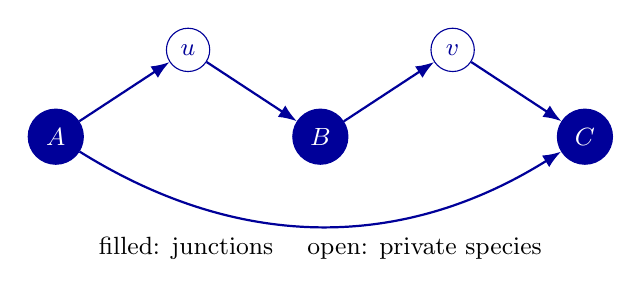
\begin{tikzpicture}[>=Latex,scale=1.05,
  jn/.style={circle,draw=blue!60!black,fill=blue!60!black,text=white,minimum size=7mm,inner sep=0pt,font=\small},
  pv/.style={circle,draw=blue!60!black,fill=white,text=blue!60!black,minimum size=5.5mm,inner sep=0pt,font=\small},
  ar/.style={->,thick,blue!60!black}]
\node[jn] (A) at (0,0) {$A$};
\node[jn] (B) at (3.2,0) {$B$};
\node[jn] (C) at (6.4,0) {$C$};
\node[pv] (u) at (1.6,1.05) {$u$};
\node[pv] (v) at (4.8,1.05) {$v$};
\draw[ar] (A)--(u); \draw[ar] (u)--(B); \draw[ar] (B)--(v); \draw[ar] (v)--(C);
\draw[ar] (A) to[bend right=32] (C);
\node[font=\small] at (3.2,-1.35) {filled: junctions \quad open: private species};
\end{tikzpicture}
\caption{A junction--path assembly with $k=3$ junctions and $M=3$ paths. Each arrow is a two-channel core~\eqref{eq:chemistry}, not a single elementary reaction. The two upper paths have private interiors; the lower path is a direct junction-to-junction core. A filled vertex has one activity in every incident path.}
\label{fig:topology}
\end{figure}

\paragraph{Relation to the predecessors.} The graded assemblies of \citep{tcch2026} are pair assemblies with unit factors admitting integer ranks that increase by one along every edge; the theorem there is sufficient only. The fans of \citep{tcch2026} and the triangle pairs of \citep{tcic2026} share one reaction and reduce to one variable. The present class has arbitrarily many species and paths, arbitrary factors, and $k$ nonlinearly interacting junction variables; unequal path lengths between the same junctions are permitted, which rules out grading (Sections~\ref{sec:linear} and~\ref{sec:operating}). The parameter $k$ is the number of remaining variables after the paths are eliminated. It is not the width of a tree decomposition of the graph, and the class is not a bounded-treewidth class.

\section{The one-edge response interval}\label{sec:edge}

For an edge with factors $a,b>0$ define the \emph{lower} and \emph{upper responses}
\begin{equation}\label{eq:responses}
  G(x)=\frac{ax+2bx^2}{a+2b},\qquad F(x)=\frac{ax+bx^2}{a+b}.
\end{equation}

\begin{lemma}[One-edge interval]\label{lem:edge}
For all real $x,y$ the core is productive at $(x_u,x_v)=(x,y)$ if and only if $G(x)<y<F(x)$. Moreover:
\begin{enumerate}[label=(\alph*)]
\item $G$ and $F$ are convex combinations of $x$ and $x^2$; they map $[0,1]$ into $[0,1]$, fix $0$ and $1$, and are strictly increasing on $[0,\infty)$;
\item for $0\le x\le y\le1$ and $c\in\{1,2\}$, with $R_c(x)=(ax+cbx^2)/(a+cb)$,
\begin{equation}\label{eq:finitediff}
  R_c(y)-R_c(x)=(y-x)\,\frac{a+cb(x+y)}{a+cb},\qquad 0<\frac{a+cb(x+y)}{a+cb}<2,
\end{equation}
so both responses are $2$-Lipschitz on $[0,1]$;
\item for $0<x<1$,
\begin{equation}\label{eq:gap}
  x^2<G(x)<F(x)<x,\qquad F(x)-G(x)=\frac{ab\,x(1-x)}{(a+b)(a+2b)}>0 .
\end{equation}
\end{enumerate}
Productivity implies $x_v<x_u$, and the answer depends on $a,b$ only through the ratio $a/b$.
\end{lemma}

\begin{proof}
Direct rearrangement of \eqref{eq:residuals} gives the two identities
\[
  2b(y-x^2)-a(x-y)=(a+2b)\bigl(y-G(x)\bigr),\qquad a(x-y)-b(y-x^2)=(a+b)\bigl(F(x)-y\bigr),
\]
with positive prefactors, which is the equivalence. Part (a) is immediate from the form of $R_c$, and (b) is a direct computation whose quotient lies in $(0,(a+2cb)/(a+cb))\subseteq(0,2)$. For (c), $R_c(x)-x^2=ax(1-x)/(a+cb)>0$ and $x-R_c(x)=cbx(1-x)/(a+cb)>0$, and the displayed difference is a direct computation. Positivity of $p_e=a(x-y)$ follows from $y<F(x)<x$. Multiplying $a$ and $b$ by a common positive constant leaves $G$ and $F$ unchanged.
\end{proof}

Scaling both factors of a core rescales its currents but not its productivity; static compatibility of a family therefore depends only on the factor ratios $a_e/b_e$, while the residual magnitudes in Section~\ref{sec:operating} do not.

\section{Exact elimination along a private path}\label{sec:path}

For a path $P=(e_1,\dots,e_r)$ in physical order put
\begin{equation}\label{eq:composed}
  G_P=G_{e_r}\circ\cdots\circ G_{e_1},\qquad F_P=F_{e_r}\circ\cdots\circ F_{e_1}.
\end{equation}
Both are strictly increasing on $[0,\infty)$, fix $0$ and $1$, and are $2^r$-Lipschitz on $[0,1]$ by Lemma~\ref{lem:edge}. A \emph{realization} of $P$ with initial value $x$ and final value $y$ is a sequence $x=t_0,t_1,\dots,t_r=y$ such that edge $e_i$ is productive at $(t_{i-1},t_i)$; it is \emph{boxed} in $[\ell,1]$ when all $t_i\in[\ell,1]$.

\begin{theorem}[Fixed-endpoint path reconstruction]\label{thm:path}
Let $\ell\le x\le1$ and $\ell\le y$. The path $P$ has a boxed realization with initial value $x$ and final value $y$ if and only if
\begin{equation}\label{eq:pathband}
  G_P(x)<y<F_P(x).
\end{equation}
When \eqref{eq:pathband} holds, a realization exists with $x=t_0>t_1>\cdots>t_r=y$, so that every interior value lies strictly between the endpoints.
\end{theorem}

\begin{proof}
\emph{Necessity.} A realization has $t_i>0$ for all $i$, since $q_{e_i}>0$ forces $t_i>t_{i-1}^2\ge0$. Lemma~\ref{lem:edge} gives $G_{e_1}(x)<t_1<F_{e_1}(x)$, and inductively, using strict monotonicity of $G_{e_{i+1}}$ and $F_{e_{i+1}}$ on $[0,\infty)$,
\[
  G_{e_{i+1}}(G_{e_i}\circ\cdots\circ G_{e_1}(x))<G_{e_{i+1}}(t_i)<t_{i+1}<F_{e_{i+1}}(t_i)<F_{e_{i+1}}(F_{e_i}\circ\cdots\circ F_{e_1}(x)).
\]
\emph{Sufficiency.} Since $G_P(1)=F_P(1)=1$, the strict band \eqref{eq:pathband} excludes $x=1$, so $0<\ell\le x<1$. For $\lambda\in[0,1]$ define the blended response $H_i(\lambda,t)=(1-\lambda)G_{e_i}(t)+\lambda F_{e_i}(t)$ and the orbit
\[
  t_0(\lambda)=x,\qquad t_i(\lambda)=H_i\bigl(\lambda,t_{i-1}(\lambda)\bigr)\quad(1\le i\le r).
\]
The endpoint $\lambda\mapsto t_r(\lambda)$ is continuous with $t_r(0)=G_P(x)$ and $t_r(1)=F_P(x)$, so by the intermediate value theorem there is $\lambda\in(0,1)$ with $t_r(\lambda)=y$. For $0<t<1$ and $0<\lambda<1$ the blend $H_i(\lambda,t)$ lies strictly inside $(G_{e_i}(t),F_{e_i}(t))$ because the gap \eqref{eq:gap} is positive, and $0<H_i(\lambda,t)<t<1$ by \eqref{eq:gap}. Inductively every $t_i(\lambda)\in(0,1)$, every edge is productive, and $x=t_0(\lambda)>t_1(\lambda)>\cdots>t_r(\lambda)=y$. All interior values lie in $(y,x)\subseteq[\ell,1]$.
\end{proof}

Theorem~\ref{thm:path} includes one-edge paths, singleton endpoint constraints and boundary equality, which is infeasible. The interpolation orbit is also the object bisected in Section~\ref{sec:algorithm} to obtain rational interior values.

\begin{remark}[Why the private box must be common]\label{rem:privatebox}
The theorem assigns interior values between the endpoints, and any realization must do so, since productivity decreases activity along every edge. An individual box on an interior species that lies entirely above the initial value $x$, or below the final value $y$, therefore makes the path infeasible even when \eqref{eq:pathband} holds. Arbitrary private boxes thus cannot be handled by the same two-function reduction; they require additional junction-like variables. This was confirmed on an exact solver control before the theorem was formalized.
\end{remark}

\begin{proposition}[Two obstructions]\label{prop:obstructions}
\leavevmode
\begin{enumerate}[label=(\roman*)]
\item A directed cycle of selected cores has no common productive state in the positive orthant, for every choice of positive factors.
\item With unit factors, the path $A\to B\to C$ and the shortcut $A\to C$ have no common productive state in the positive orthant. Writing $G(x)=(x+2x^2)/3$ and $F(x)=(x+x^2)/2$,
\begin{equation}\label{eq:shortcut}
  G(x)-F(F(x))=\frac{x(1-x)(3x^2+9x+2)}{24}>0\qquad(0<x<1).
\end{equation}
\end{enumerate}
\end{proposition}

\begin{proof}
(i) Productivity decreases activity along every edge, and a cycle would return to its starting species. (ii) A productive edge with positive activities forces $x_A<1$ by \eqref{eq:gap}. The two-edge path requires $x_C<F(F(x_A))$ by Theorem~\ref{thm:path}, the shortcut requires $x_C>G(x_A)$, and \eqref{eq:shortcut} is an exact polynomial identity.
\end{proof}

Part (ii) is the $n=3$ case of the unbounded-order conflict of \citep{tcch2026}; it is an exact negative control, not a failure of a local numerical search. Acyclicity alone is therefore not sufficient for compatibility, and Section~\ref{sec:operating} shows that the same graph becomes compatible for other factors.

\section{The junction--path compatibility theorem}\label{sec:assembly}

\begin{theorem}[Junction--path compatibility]\label{thm:main}
Let a junction--path assembly with arbitrary positive real factors and boxes $[l_j,u_j]\subseteq[\ell,1]$ be given. There is an activity vector $x\in\R^V$ with $x_s\in[\ell,1]$ for all $s$, $x_j\in[l_j,u_j]$ for all $j\in J$, and every selected core productive, if and only if there is a vector $z\in\R^J$ with
\begin{equation}\label{eq:reduced}
  l_j\le z_j\le u_j\quad(j\in J),\qquad G_P(z_{s(P)})<z_{t(P)}<F_P(z_{s(P)})\quad(P=P_1,\dots,P_M).
\end{equation}
The inequalities \eqref{eq:reduced} are inequalities on the actual shared species: a junction has one variable, not one copy per incident path.
\end{theorem}

\begin{proof}
If $x$ is a common productive state, its restriction to each path is a boxed realization between the junction values, so Theorem~\ref{thm:path} gives \eqref{eq:reduced} with $z=x|_J$. Conversely fix a feasible $z$. For each path apply Theorem~\ref{thm:path} with initial value $z_{s(P)}$ and final value $z_{t(P)}$; both lie in $[\ell,1]$ because the junction boxes are subboxes of $[\ell,1]$. Define $x_j=z_j$ on junctions and $x_s$ equal to the constructed value of the unique occurrence of $s$ on the unique path containing a private species $s$; give isolated species the value $\ell$. Condition (ii) of Definition~\ref{def:class} makes this single-valued, and every occurrence of a junction on a path is an endpoint whose constructed value equals $z_j$ by construction. Every selected core is productive at $x$ and all boxes hold. Finally, the identities \eqref{eq:currents}--\eqref{eq:residuals} identify the edge statements with the source-level predicate that the motif of $e$ is productive for the current vector \eqref{eq:current} of the literal network, and every motif is a PAC.
\end{proof}

The identification in the last sentence, from the abstract edge inequalities back to the reversible network with activity monomials, is where the formal statement lives: the Lean theorem \lean{sourceCompatible_iff_junctionFeasible} (Section~\ref{sec:formal}) is stated for a structure that records the paths, the placement of path positions on species, the junction predicate, the endpoint characterization and private uniqueness, and asserts the equivalence between the source-level compatibility predicate and the feasibility of \eqref{eq:reduced}. The merge step is a separate compiled lemma that produces one global vector from local path vectors agreeing on junctions.

\begin{corollary}\label{cor:real}
For $k=0$ a valid assembly has no paths, and every vector in the boxes is compatible. For $k\ge1$ compatibility is a semialgebraic condition on $z\in\R^k$ defined by $2M$ strict polynomial inequalities of degree at most $2^h$ and $2k$ weak linear ones.
\end{corollary}

\section{A complete rational algorithm with a bit bound}\label{sec:algorithm}

Assume now that all factors, $\ell$ and all box endpoints are rational, let $B\ge1$ bound the bit lengths of their numerators and denominators, and let $n$ bound the explicit input size (species, edges, path lists and their labels). Put $D=2^h$.

\subsection{The external decision routine}\label{sec:backend}

We use the one-block quantifier-elimination theorem of Basu, Pollack and Roy in the form stated in Basu's survey \citep[Theorem 2.27]{basu2014}, \citep[Chapter 14]{bpr2006}: for a formula with at most $s$ polynomials of degree at most $d$ in one block of $k$ quantified variables and $\ell_{\mathrm f}$ free variables, an equivalent quantifier-free formula is computed with $s^{(k+1)(\ell_{\mathrm f}+1)}d^{O(k)O(\ell_{\mathrm f})}$ arithmetic operations, and if the coefficients are integers of bit size at most $\tau$, then all intermediate and output integers have bit size at most $\tau d^{O(k)O(\ell_{\mathrm f})}$. We use $\ell_{\mathrm f}\in\{0,1\}$; a pure decision may be treated as having one unused free variable, so that in both roles the operation count is $(s(d+1))^{O(k+1)}$ and the integer height is $\tau(d+1)^{O(k+1)}$. Earlier singly exponential procedures \citep{grigoriev1988,renegar1992} would serve equally; cylindrical algebraic decomposition \citep{collins1975} and Tarski's original method \citep{tarski1951} are complete but have worse bounds. This is the only external algorithm the theorem depends on, and the contribution here is the reduction to it and the control of the rational output, not the elimination itself.

\subsection{The algorithm}\label{sec:steps}

Let $f_1,\dots,f_{2M}$ denote the $2M$ response residuals $z_{t(P)}-G_P(z_{s(P)})$ and $F_P(z_{s(P)})-z_{t(P)}$, with positive denominators cleared so that each is an integer polynomial in $z$.
\begin{enumerate}[label=\textbf{Step \arabic*.},leftmargin=*,align=left]
\item \emph{Validate.} Check the graph, factors, boxes, path orientation and continuity, endpoint membership in $J$, private uniqueness and edge coverage; reject malformed data. If $E=\emptyset$, return box midpoints for junctions and $\ell$ elsewhere.
\item \emph{Reduce.} Construct $G_P,F_P$ for every path by rational polynomial composition (Lemma~\ref{lem:representation}). Decide \eqref{eq:reduced}. If infeasible, return \textsc{incompatible}.
\item \emph{Slack.} For $t=1,\tfrac12,\tfrac14,\dots$ decide whether the boxes together with $f_i\ge t$ for all $i$ are feasible; keep the first success $t_0$ (Lemma~\ref{lem:slack}).
\item \emph{Junction brackets.} Maintain one closed rational bracket per junction, initially its box, with the invariant that some real vector in the product of brackets satisfies all $f_i\ge t_0$. Repeatedly bisect a bracket and decide whether its left closed half, the other current brackets and all $f_i\ge t_0$ are jointly feasible; keep the left half if so, otherwise the right half. Stop when all widths are at most $\eta=t_0/(4(D+1))$ (Lemma~\ref{lem:precision}).
\item \emph{Private reconstruction.} Take the bracket midpoints as junction activities. For each path of length at least two, bisect the interpolation parameter of Theorem~\ref{thm:path} with exact rational arithmetic until the last edge is productive with the prescribed final value (Lemma~\ref{lem:bisection}).
\item \emph{Check and output.} Merge by species identity, evaluate every current and residual exactly, verify every box, and output the rational state.
\end{enumerate}

\begin{theorem}[Complete rational decision and reconstruction]\label{thm:algorithm}
Steps 1--6 decide every validated rational instance and, when feasible, output a rational common productive state. The total bit cost and the output length are bounded by
\begin{equation}\label{eq:complexity}
  \Abound^{O(k+1)},\qquad \Abound=(n+M+k+2)(2^h+1)(B+h+1).
\end{equation}
For fixed $k$ and $h\le C\log_2(n+2)$ with fixed $C$ this is polynomial in the binary input size.
\end{theorem}

The remainder of this section proves the four lemmas that the steps rely on and then assembles the bound. Table~\ref{tab:precision} collects the quantities.

\subsection{Response representation}

\begin{lemma}[Positive representation]\label{lem:representation}
Write $a=A_1/A_2$ and $b=B_1/B_2$ in positive integers and put $\alpha=A_1B_2$, $\beta=B_1A_2$. Represent a composed response as $N(X)/Q$ with an integer polynomial $N$ and a positive integer $Q$. Appending an edge with lower ($c=2$) or upper ($c=1$) response gives
\begin{equation}\label{eq:recurrence}
  N_{\mathrm{new}}=\alpha QN+c\beta N^2,\qquad Q_{\mathrm{new}}=(\alpha+c\beta)Q^2 .
\end{equation}
Starting from $N=X$, $Q=1$, every numerator has nonnegative coefficients summing to $Q$; hence each coefficient is at most $Q$. After $r$ edges the degree is exactly $2^r$, and if all input numerators and denominators are below $2^B$ then $\log_2Q<(2^r-1)(2B+2)$. Consequently every composed response has degree at most $D$ and integer height $\tau=O(D(B+1))$, and constructing both responses of every path by dense schoolbook arithmetic costs a polynomial in $M$, $D$ and $B$. Clearing the positive denominators turns \eqref{eq:reduced} into $s=O(M+k+1)$ integer polynomial constraints in $k$ variables of degree at most $D$ and height $O(\tau)$, in a formula of length linear in $s$.
\end{lemma}

\begin{proof}
Substituting $N/Q$ into $(\alpha x+c\beta x^2)/(\alpha+c\beta)$ gives \eqref{eq:recurrence}. If $N$ has nonnegative coefficients with $N(1)=Q$, then $N_{\mathrm{new}}$ has nonnegative coefficients and $N_{\mathrm{new}}(1)=\alpha Q^2+c\beta Q^2=Q_{\mathrm{new}}$. Leading coefficients are positive, so the degree doubles. From $\alpha+c\beta<2^{2B+2}$ the recurrence $\log_2Q_{\mathrm{new}}=\log_2(\alpha+c\beta)+2\log_2Q$ gives the stated bound. The remaining statements are direct.
\end{proof}

The representation is not reduced by greatest common divisors, and the bound is a property of this representation: for $a=b=1$ and the upper response the reduced leading coefficient after $r$ edges is $2^{-(2^r-1)}$, so the exponential height is intrinsic to the expanded polynomial, while no hardness for other algorithms follows.

\subsection{A dyadic slack with a proved search bound}

\begin{lemma}[Slack]\label{lem:slack}
Suppose \eqref{eq:reduced} is feasible. Then there is a universal constant $c_0$ such that with
\begin{equation}\label{eq:H}
  H=\tau(D+1)^{c_0(k+1)}
\end{equation}
every $t\in(0,2^{-(H+2)})$ is a feasible slack, i.e.\ the boxes and $f_i\ge t$ for all $i$ are jointly satisfiable. Hence Step~3 succeeds within $H+3$ decisions.
\end{lemma}

\begin{proof}
Consider the formula with quantified block $z\in\R^k$ and one free variable $t$: the boxes, $f_i(z)\ge t$ for all $i$, and $0<t\le1$. By the backend theorem an equivalent quantifier-free formula $\Psi(t)$ exists whose polynomials have integer coefficients of bit size at most $H$ as in \eqref{eq:H}, for a suitable universal $c_0$. Discard identically zero polynomials, whose signs are constant, and divide every remaining polynomial by its largest power of $t$, which does not change signs on $t>0$; its constant coefficient is then a nonzero integer of absolute value at least one. By the reciprocal Cauchy bound \citep{mignotte1992}, every nonzero root of an integer polynomial with constant term $c_0'\neq0$ and coefficients of absolute value at most $2^H$ has absolute value at least $|c_0'|/(|c_0'|+2^H)>2^{-(H+1)}$. Hence no polynomial of $\Psi$ changes sign on $(0,2^{-(H+2)})$ and the truth value of $\Psi$ is constant there. The set of feasible slacks is nonempty, since a strictly feasible $z$ has a positive minimum residual, and it is downward closed in $(0,1]$; so it meets $(0,2^{-(H+2)})$, and by constancy contains it. The dyadic sequence $2^{-i}$ enters that interval at $i=H+3$.
\end{proof}

The elimination with a free variable is used only to bound the number of decisions actually executed. The algorithm itself never constructs $\Psi$, isolates a root or guesses a chemical margin.

\subsection{Rational junction coordinates}

\begin{lemma}[Junction precision]\label{lem:precision}
Each composed response is $D$-Lipschitz on $[0,1]$, so every residual $f_i$ has Lipschitz constant at most $D+1$ with respect to the maximum norm on the box. Step~4 preserves the invariant that one real vector in the product of the current brackets has all residuals at least $t_0$; when all widths are at most $\eta=t_0/(4(D+1))$, the vector $z^\circ$ of bracket midpoints satisfies every residual $f_i(z^\circ)\ge 3t_0/4>0$ and lies exactly in every original box, including singleton boxes. Each coordinate needs $O(H+h+1)$ decisions, and the rational midpoints have bit length $L=O(B+H+h+1)$.
\end{lemma}

\begin{proof}
The Lipschitz bound composes \eqref{eq:finitediff} at most $h$ times. If the left closed half of a bracket, together with the other brackets and the residual constraints, is infeasible, then the witness guaranteed by the invariant lies in the right closed half, because the two closed halves cover the parent bracket; so the invariant is preserved either way, and it holds initially by Step~3. At the end some real witness $w$ lies in all final brackets, so $\|z^\circ-w\|_\infty\le\eta$ and $f_i(z^\circ)\ge t_0-(D+1)\eta=3t_0/4$. Midpoints of closed subbrackets of the boxes lie in the boxes; a singleton box is never bisected. A bracket of initial width at most one reaches width $\eta$ after $\lceil\log_2(1/\eta)\rceil=O(\log(1/t_0)+h)=O(H+h+1)$ bisections by Lemma~\ref{lem:slack}, and its endpoints are dyadic refinements of $B$-bit rationals.
\end{proof}

Retaining brackets rather than fixing a rational value for one coordinate before the others are refined is essential: a prematurely fixed coordinate may destroy the common witness for the remaining strict inequalities.

\subsection{Rational private reconstruction}

\begin{lemma}[Rational bisection]\label{lem:bisection}
Let $P$ have length $r\ge2$ and rational endpoints $\ell\le y<x<1$ with $G_P(x)<y<F_P(x)$. Put
\[
  \delta=\min\{y-G_P(x),\,F_P(x)-y\}>0,\qquad C=2^r-1,\qquad C'=2^{r-1}-1 .
\]
Let $E(\lambda)=t_r(\lambda)$ and $T(\lambda)=t_{r-1}(\lambda)$ be the full and prefix endpoints of the interpolation orbit of Theorem~\ref{thm:path}, and let $a,b$ be the factors of the last edge. Then
\begin{enumerate}[label=(\alph*)]
\item $E$ and $T$ are strictly increasing on $[0,1]$ with Lipschitz constants $C$ and $C'$ in $\lambda$;
\item if $E(\lambda_*)=y$ then $\lambda_*,1-\lambda_*\ge\delta/C$, $y<T(\lambda_*)<x$, and the last-edge gap at $T(\lambda_*)$ is at least $\gamma=ab\ell(1-x)/((a+b)(a+2b))>0$, so both last-edge margins $y-G(T(\lambda_*))$ and $F(T(\lambda_*))-y$ are at least $m=\delta\gamma/C$;
\item every rational $\lambda\in(0,1)$ with $|\lambda-\lambda_*|<m/(4C')$ makes all prefix edges productive along the orbit and the last edge productive at $(T(\lambda),y)$.
\end{enumerate}
Consequently bisection of $[0,1]$ on the sign of $E(\lambda)-y$, testing the last edge with the prescribed $y$ at each midpoint, terminates within $1+\lceil\log_2(4CC'/(\delta\gamma))\rceil=O(D(B+L)+h+1)$ iterations, and the private values it produces have bit length $O(D^2(B+L+h+1))$.
\end{lemma}

\begin{proof}
(a) Each blend $H_i(\lambda,t)$ is $2$-Lipschitz in $t$ by \eqref{eq:finitediff} and $1$-Lipschitz in $\lambda$ because $0\le F_{e_i}(t)-G_{e_i}(t)\le1$ on $[0,1]$; induction gives the constants $\sum_{i<r}2^i=C$ and $C'$. The first blend is strictly increasing in $\lambda$ for $x\in(0,1)$ by \eqref{eq:gap}, and every later map is strictly increasing in its input and nondecreasing in $\lambda$. (b) From $E(0)=G_P(x)$, $E(1)=F_P(x)$ and the Lipschitz bound, $\delta\le|E(\lambda_*)-E(0)|\le C\lambda_*$, and likewise for $1-\lambda_*$. The orbit is strictly decreasing, so $y<T(\lambda_*)<x$, and \eqref{eq:gap} evaluated at $T(\lambda_*)\in[\ell,x]$ is at least $\gamma$. Since $y=(1-\lambda_*)G(T(\lambda_*))+\lambda_*F(T(\lambda_*))$, the two margins are $\lambda_*$ and $1-\lambda_*$ times the gap. (c) The functions $\lambda\mapsto G(T(\lambda))$ and $F(T(\lambda))$ are $2C'$-Lipschitz, so within $m/(4C')$ of $\lambda_*$ both last-edge inequalities lose less than $m/2$ of their margin and stay strict; prefix edges are productive for every $\lambda\in(0,1)$ by Theorem~\ref{thm:path}. Bisection retains a bracket containing $\lambda_*$; once its length is below $m/(4C')$ its midpoint passes, and equality $E(\lambda)=y$ passes immediately. The rational numbers defining $\delta$ have bit length $O(D(B+L))$ by Lemma~\ref{lem:representation}, $\gamma$ has bit length $O(B+L)$, and $\log_2(CC')=O(h)$, which gives the iteration bound. A bisection parameter has that many bits, and evaluating the quadratic orbit $r\le h$ times multiplies bit lengths by at most $2^r\le D$.
\end{proof}

One-edge paths need no reconstruction. The lemma replaces root isolation in a compositum of the path fields by exact bisection with an explicit last-edge margin.

\subsection{Assembling the bound}

\begin{proof}[Proof of Theorem~\ref{thm:algorithm}]
\emph{Correctness.} Step~2 is Theorem~\ref{thm:main} together with Corollary~\ref{cor:real}. If it succeeds, Step~3 terminates by Lemma~\ref{lem:slack}, Step~4 produces junction values in the boxes with all residuals positive by Lemma~\ref{lem:precision}, and Step~5 produces a boxed realization of every path with those endpoints by Lemma~\ref{lem:bisection}. The merge of Theorem~\ref{thm:main} is single-valued, and Step~6 is an exact recheck of the literal currents, boxes and residuals, so the output is a certified common productive state. If Step~2 fails, no common state exists by Theorem~\ref{thm:main}.

\emph{Cost.} The number of decisions in Steps~2--4 is $Q_*=O((k+1)(H+B+h+1))$ by Lemmas~\ref{lem:slack} and~\ref{lem:precision}. Every decision has $O(M+k+1)$ polynomials of degree at most $D$ with integer coefficients of bit size
\[
  T_q=O(\tau+B+H+h+1),
\]
which includes the cleared response denominators, the current slack and the current bracket endpoints. By the backend bound a decision costs at most $(s(D+1))^{c(k+1)}\bigl[T_q(D+1)^{c'(k+1)}\bigr]^2$ bit operations for universal $c,c'$, the square accounting for schoolbook integer arithmetic on intermediate integers of that size. The height $T_q$ enters with a fixed exponent; substituting \eqref{eq:H} and multiplying by $Q_*$ therefore leaves an exponent $O(k+1)$ rather than $O(k^2)$. Validation is polynomial in $n$ and $B$ with a sorting step for edge coverage; response construction is polynomial in $M,D,B$ by Lemma~\ref{lem:representation}; private reconstruction of $M$ paths is polynomial in $D,B,L$ by Lemma~\ref{lem:bisection}; the exact check and the output of $O(n)$ rational values of bit length $O(D^2(B+L+h+1))$ are polynomial in the same quantities. All of these are bounded by \eqref{eq:complexity}. For $k=0$ a valid assembly has no paths, and the empty-edge case is handled in Step~1 without any decision. For fixed $k$ and $h\le C\log_2(n+2)$, $D$ is polynomial in $n$ and the exponent is fixed.
\end{proof}

\begin{table}[t]
\centering\small
\begin{tabular}{@{}ll@{}}\toprule
Quantity & Bound \\\midrule
Response degree; integer height & $D=2^h$; $\tau=O(D(B+1))$ \\
Constraints per decision & $s=O(M+k+1)$ \\
Slack-elimination height & $H=\tau(D+1)^{O(k+1)}$ \\
Dyadic slack & $t_0>2^{-(H+3)}$ \\
Decisions in Steps 2--4 & $Q_*=O((k+1)(H+B+h+1))$ \\
Integer height per decision & $T_q=O(\tau+B+H+h+1)$ \\
Junction bits per coordinate & $L=O(B+H+h+1)$ \\
Bisection iterations per path & $O(D(B+L)+h+1)$ \\
Private bits per coordinate & $O(D^2(B+L+h+1))$ \\\bottomrule
\end{tabular}
\caption{Precision and size accounting for Theorem~\ref{thm:algorithm}. Heights count bits of numerators and denominators or of integer coefficients, as appropriate.}
\label{tab:precision}
\end{table}

\subsection{An executable demonstration}\label{sec:demo}

The proofs above specify the one-block elimination routine as the decision backend. A small executable in the accompanying repository answers the same reduced formulas with the exact nonlinear real arithmetic solver of Z3 \citep{demoura2008,jovanovic2012} in place of that routine, performs the dyadic slack search, the bracket bisection and the private bisection exactly as in Steps~3--5, rechecks every output with exact rational arithmetic, and reports \textsc{unknown} rather than a verdict when a query times out. The worst-case bound of Theorem~\ref{thm:algorithm} is not asserted for this backend. Table~\ref{tab:demo} lists its regression on eight fixtures for the graph of Figure~\ref{fig:responses}; the run used 93 queries and about $0.15$ seconds in total (Windows, Python 3.11, Z3 4.15, a 3-second per-query limit), which is a demonstration measurement rather than a benchmark.

\begin{table}[t]
\centering\footnotesize
\begin{tabular}{@{}>{\raggedright\arraybackslash}p{.30\linewidth}lr>{\raggedright\arraybackslash}p{.40\linewidth}@{}}\toprule
Fixture & Verdict & Queries & Output or reason \\\midrule
three junctions, factors $(9,1),(9,1),(2,1)$ & \textsc{sat} & 45 & $(37859/40960,\,37379/40960,\,7373/8192)$, slack $1/1024$ \\
same graph, $B$ private on the path $A\to B\to C$ & \textsc{sat} & 31 & $x_B=6746098527/7381975040$, $\lambda=1/4$ after two bisections \\
unit factors & \textsc{unsat} & 1 & Proposition~\ref{prop:obstructions}(ii) \\
singleton boxes at \eqref{eq:witness} & \textsc{sat} & 15 & the state \eqref{eq:witness} itself, slack $1/8192$ \\
directed cycle & \textsc{unsat} & 1 & Proposition~\ref{prop:obstructions}(i) \\
path listed against its orientation & \textsc{invalid} & 0 & orientation/discontinuity \\
box with lower bound above upper bound & \textsc{invalid} & 0 & invalid junction box \\
four junctions with bound $k\le3$ & \textsc{outside} & 0 & class bound exceeded \\\bottomrule
\end{tabular}
\caption{Eight-fixture regression of the executable demonstration. Every \textsc{sat} output was rechecked exactly. The first output is a different rational witness from \eqref{eq:witness} for the same assembly; the second reconstructs the private species with certified last-edge margin $4137432795063009099/4219980937237211643904000$ and a proved budget of 21 iterations.}
\label{tab:demo}
\end{table}

Two further small pilots test the lemmas rather than the theorem. The representation recurrence \eqref{eq:recurrence} was run up to $h=8$: the degree and denominator bit length were exactly $2,4,16,256$ for $h=1,2,4,8$ with unit factors, and $52,144,504$ denominator bits for $h=4$ with input heights $B=2,8,32$, matching Lemma~\ref{lem:representation}. The bisection of Lemma~\ref{lem:bisection} was run on eighteen paths of lengths $2,3,5$ with target endpoints at relative positions $10^{-4}$, $1/2$ and $1-10^{-4}$ of the band; the largest observed iteration count was $14$ against a largest proved budget of $43$. Narrowing the band of the three-junction instance by factors $10$, $10^3$ and $10^5$ raised the query count from $15$ to $22$ to $28$, with slacks $2^{-13}$, $2^{-20}$ and $2^{-26}$. None of this is evidence for the universal statements, which are proved above; it checks that the implemented recurrences and searches behave as the proofs predict.

\section{A constructive linear sufficient class}\label{sec:linear}

The exact residual identities also yield a fast sufficient construction that does not need the junction--path structure at all. Write activities as deficits from the equilibrium point,
\[
  x_s=1-\varepsilon d_s,\qquad d_s>0,\qquad \alpha_e=\frac{a_e+2b_e}{a_e+b_e},\qquad \beta_e=\frac{a_e+4b_e}{a_e+2b_e}.
\]
Note $1<\alpha_e<\beta_e<2$.

\begin{proposition}[Finite-deficit certificate]\label{prop:linear}
Suppose $\alpha_ed_u<d_v<\beta_ed_u$ on every selected edge $e\colon u\to v$, and put
\[
  U_e=(a_e+4b_e)d_u-(a_e+2b_e)d_v>0,\qquad V_e=(a_e+b_e)d_v-(a_e+2b_e)d_u>0 .
\]
If
\begin{equation}\label{eq:eps}
  0<\varepsilon<\min_e\frac{U_e}{2b_ed_u^2}\qquad\text{and}\qquad \varepsilon\max_s d_s\le1-\ell,
\end{equation}
then $x$ lies in $[\ell,1]^V$ and makes every selected core productive. A junction box $[l_s,u_s]$ additionally requires $(1-u_s)/d_s\le\varepsilon\le(1-l_s)/d_s$.
\end{proposition}

\begin{proof}
Substituting into \eqref{eq:residuals} gives the exact expansions, with no discarded remainder,
\begin{equation}\label{eq:deficit}
  \ru=\varepsilon U_e-2b_e\varepsilon^2d_u^2,\qquad \rv=\varepsilon V_e+b_e\varepsilon^2d_u^2 .
\end{equation}
The first is positive exactly when $\varepsilon<U_e/(2b_ed_u^2)$, the second whenever $V_e>0$. The box conditions are direct.
\end{proof}

For rational data the strict homogeneous system $\alpha_ed_u<d_v<\beta_ed_u$, $d_s>0$ is decided by one rational linear program: normalize $\sum_sd_s=1$, maximize $t$ subject to $d_s\ge t$, $d_v-\alpha_ed_u\ge t$ and $\beta_ed_u-d_v\ge t$. The optimum is positive exactly when the strict system is feasible, and an optimal basic solution is rational of polynomial bit length \citep{khachiyan1979,schrijver1986}. The bounds \eqref{eq:eps} and the box constraints are then finitely many rational intervals in $\varepsilon$, whose intersection is computed in polynomial time. Without junction boxes the intersection is nonempty whenever the linear program is positive; with junction boxes it may be empty for the returned deficits, and the procedure is then a sufficient test for those deficits rather than an optimization over all of them. A failed certificate does not prove incompatibility. Since $\alpha_e>1$, a directed cycle never passes.

\paragraph{A nongraded unit-factor assembly.} With $a_e=b_e=1$ the ratio interval is $(3/2,5/3)$. Two paths between the same pair of junctions with lengths $r<r'$ can both satisfy the strict ratio criterion only if $(3/2)^{r'}<(5/3)^{r}$; lengths $3$ and $4$ fail, and $4$ and $5$ are the first adjacent lengths that succeed, since $(3/2)^5=7.59\ldots<7.71\ldots=(5/3)^4$. Take
\begin{align*}
  d^{(4)}&=\bigl(1,\ \tfrac{83}{50},\ \tfrac{69}{25},\ \tfrac{459}{100},\ \tfrac{191}{25}\bigr),\\
  d^{(5)}&=\bigl(1,\ \tfrac{1501}{1000},\ \tfrac{1127}{500},\ \tfrac{3383}{1000},\ \tfrac{1269}{250},\ \tfrac{191}{25}\bigr),
\end{align*}
sharing their first and last entries, and $\varepsilon=10^{-4}$. Every adjacent ratio lies strictly in $(3/2,5/3)$, all activities lie in $[9/10,1]$, and exact evaluation of \eqref{eq:deficit} over the nine cores gives minimum production $21/10^8>0$. The assembly has nine species (two junctions and seven private species), nine cores and two junctions (Figure~\ref{fig:nongraded}). An integer rank increasing by one on every core would assign both $4$ and $5$ to the same pair of junctions, so no grading exists, and the graded certificate of \citep{tcch2026} cannot produce this state. No minimality claim is made for this example; the six-and-seven-edge version was found first.

\begin{figure}[t]
\centering
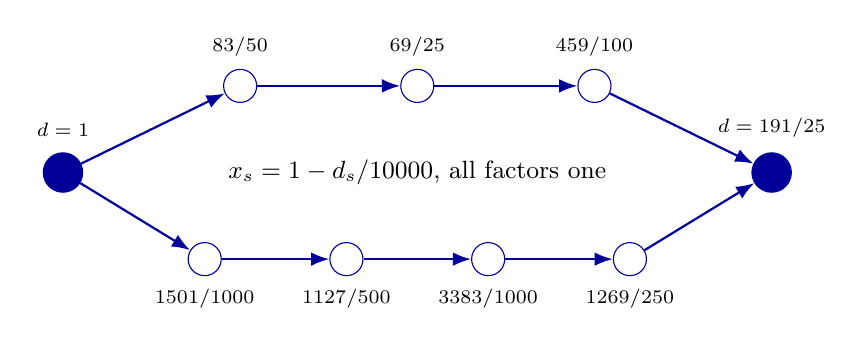
\begin{tikzpicture}[>=Latex,scale=1.0,
  jn/.style={circle,draw=blue!60!black,fill=blue!60!black,minimum size=5mm,inner sep=0pt},
  pv/.style={circle,draw=blue!60!black,fill=white,minimum size=4.2mm,inner sep=0pt},
  ar/.style={->,thick,blue!60!black},lab/.style={font=\scriptsize}]
\node[jn] (s) at (0,0) {}; \node[lab,above=2pt of s] {$d=1$};
\node[jn] (t) at (9,0) {}; \node[lab,above=2pt of t] {$d=191/25$};
\node[pv] (a1) at (2.25,1.1) {}; \node[lab,above=1pt of a1] {$83/50$};
\node[pv] (a2) at (4.5,1.1) {};  \node[lab,above=1pt of a2] {$69/25$};
\node[pv] (a3) at (6.75,1.1) {}; \node[lab,above=1pt of a3] {$459/100$};
\node[pv] (b1) at (1.8,-1.1) {}; \node[lab,below=1pt of b1] {$1501/1000$};
\node[pv] (b2) at (3.6,-1.1) {}; \node[lab,below=1pt of b2] {$1127/500$};
\node[pv] (b3) at (5.4,-1.1) {}; \node[lab,below=1pt of b3] {$3383/1000$};
\node[pv] (b4) at (7.2,-1.1) {}; \node[lab,below=1pt of b4] {$1269/250$};
\draw[ar] (s)--(a1); \draw[ar] (a1)--(a2); \draw[ar] (a2)--(a3); \draw[ar] (a3)--(t);
\draw[ar] (s)--(b1); \draw[ar] (b1)--(b2); \draw[ar] (b2)--(b3); \draw[ar] (b3)--(b4); \draw[ar] (b4)--(t);
\node[font=\small] at (4.5,0) {$x_s=1-d_s/10000$, all factors one};
\end{tikzpicture}
\caption{The unit-factor four/five assembly. Labels are the exact deficits; the two junctions are shared. The displayed rational state makes all nine cores productive in $[9/10,1]$ with minimum production $21/10^8$, although no integer grading of the graph exists.}
\label{fig:nongraded}
\end{figure}

\section{Operating certificates at a weighted example}\label{sec:operating}

Throughout this section use the three cores $A\to B$, $B\to C$ and $A\to C$ of Proposition~\ref{prop:obstructions}(ii), now with factors and state
\begin{equation}\label{eq:witness}
\begin{aligned}
  (a,b)_{AB}&=(9,1),\qquad (a,b)_{BC}=(9,1),\qquad (a,b)_{AC}=(2,1),\\
  (x_A,x_B,x_C)&=\Bigl(\frac{99}{100},\ \frac{593}{600},\ \frac{3551}{3600}\Bigr).
\end{aligned}
\end{equation}
All activities lie in $[9/10,1]$. Table~\ref{tab:currents} gives the exact currents; every residual is positive, with minimum $7/7500$ on the target side of the shortcut. The state also arises from Proposition~\ref{prop:linear} with $d=(1,7/6,49/36)$ and $\varepsilon=1/100$, whose $U_e,V_e$ are positive and satisfy \eqref{eq:eps}. Figure~\ref{fig:responses} shows the composed responses of the two-edge path and of the shortcut: their bands overlap, whereas with unit factors they never do by \eqref{eq:shortcut}. The rank equations $r_B=r_A+1$, $r_C=r_B+1$, $r_C=r_A+1$ are inconsistent, so this compatible assembly is also nongraded.

\begin{table}[t]
\centering\renewcommand{\arraystretch}{1.8}
\begin{tabular}{@{}lrrrrr@{}}\toprule
Edge & $p_e$ & $q_e$ & $2q_e-p_e$ & $p_e-q_e$ & $\rho_e$ \\\midrule
$AB$ & $\frac{3}{200}$ & $\frac{247}{30000}$ & $\frac{11}{7500}$ & $\frac{203}{30000}$ & $\frac{11}{236}$ \\
$BC$ & $\frac{7}{400}$ & $\frac{3451}{360000}$ & $\frac{301}{180000}$ & $\frac{2849}{360000}$ & $\frac{43}{943}$ \\
$AC$ & $\frac{13}{1800}$ & $\frac{283}{45000}$ & $\frac{241}{45000}$ & $\frac{7}{7500}$ & $\frac{21}{304}$ \\
\bottomrule\end{tabular}

\caption{Exact currents, residuals and per-edge relative-factor radii $\rho_e$ of Proposition~\ref{prop:relative} at the state~\eqref{eq:witness}, food activity one. Every residual is strictly positive.}
\label{tab:currents}
\end{table}

\begin{figure}[t]
\centering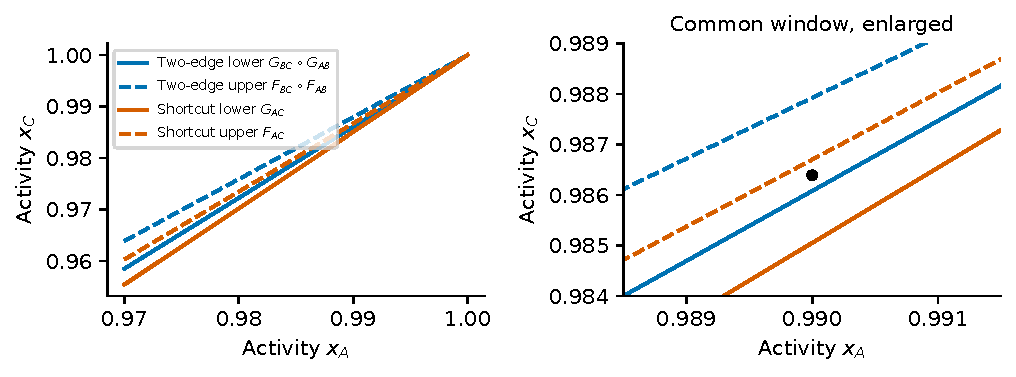
\includegraphics[width=\linewidth]{figures/responses.pdf}
\caption{Composed responses for the weighted example. The band of the two-edge path $A\to B\to C$ (blue) and the band of the shortcut $A\to C$ (orange) overlap; the black point is the exact endpoint pair $(x_A,x_C)$ of~\eqref{eq:witness}. Curves are sampled for display from the exact formulas; the certificate is rational.}
\label{fig:responses}
\end{figure}

Holding all three activities, $b_{AC}=1$ and the two other cores fixed, the shortcut is productive exactly when $q_{AC}<a_{AC}(x_A-x_C)<2q_{AC}$, i.e.
\[
  \frac{566}{325}<a_{AC}<\frac{1132}{325}.
\]
This slice does not contradict the unit-factor incompatibility, which changes $a_{AB}$ and $a_{BC}$ as well.

\subsection{Sharp relative-factor tolerance}

\begin{proposition}[Independent relative uncertainty]\label{prop:relative}
Fix a productive state with nonempty edge set and let each factor vary independently in $[(1-\rho)a_e,(1+\rho)a_e]$ and $[(1-\rho)b_e,(1+\rho)b_e]$, $0\le\rho<1$. Every core stays strictly productive throughout the whole factor box if and only if $\rho<\rho_*$, where
\begin{equation}\label{eq:radius}
  \rho_*=\min_{e\in E}\rho_e,\qquad \rho_e=\min\Bigl\{\frac{2q_e-p_e}{2q_e+p_e},\ \frac{p_e-q_e}{p_e+q_e}\Bigr\},
\end{equation}
with $p_e,q_e$ the nominal currents.
\end{proposition}

\begin{proof}
With factor multipliers $u,v\in[1-\rho,1+\rho]$ the residuals become $2vq_e-up_e$ and $up_e-vq_e$, affine in $(u,v)$ with $p_e,q_e>0$. The first is minimized at $(u,v)=(1+\rho,1-\rho)$ with value $2q_e-p_e-\rho(2q_e+p_e)$, the second at the opposite corner with value $p_e-q_e-\rho(p_e+q_e)$. Both minima are positive exactly when $\rho<\rho_e$, and at $\rho=\rho_e$ a corner has a zero residual, so the threshold is attained.
\end{proof}

At \eqref{eq:witness} the three radii are $11/236$, $43/943$ and $21/304$ (Table~\ref{tab:currents}), so $\rho_*=43/943\simeq0.0456$, set by the source side of $B\to C$. At $\rho=1/25$ every residual throughout the factor box is at least $77/375000$. For absolute perturbations $|a'_e-a_e|,|b'_e-b_e|\le\rho$ one has $|p'-p|,|q'-q|\le\rho$ on $[0,1]^2$, hence residual changes at most $3\rho$; at $\rho=10^{-4}$ every residual stays at least $7/7500-3\cdot10^{-4}=19/30000$. Sharpness concerns the fixed state; a state reoptimized after perturbation could tolerate more.

\subsection{Joint activity, factor and food rectangles}

Let activities range independently in positive intervals $[L_s,U_s]$, factors in positive intervals, and the food activity in $[f_-,f_+]$ with $f_->0$. Then $p=a(x-y)$, $q=b(fy-x^2)$ and
\begin{equation}\label{eq:foodres}
  r_u=-2bx^2-ax+(a+2bf)y,\qquad r_v=bx^2+ax-(a+bf)y .
\end{equation}

\begin{proposition}[Eight-corner certificate]\label{prop:corner}
Every core is productive throughout the whole rectangle if and only if, for every edge $e\colon u\to v$, $r_u>0$ at $(x,y,f)=(U_u,L_v,f_-)$ for each of the four factor corners, and $r_v>0$ at $(x,y,f)=(L_u,U_v,f_+)$ for each of the four factor corners.
\end{proposition}

\begin{proof}
For nonnegative factors, activities and food, $r_u$ is nonincreasing in $x$ and nondecreasing in $y$ and $f$, and $r_v$ has the opposite monotonicities, so each is minimized over the activity/food rectangle at the stated corner. At fixed $(x,y,f)$ each residual is affine in $(a,b)$, so its minimum over the factor rectangle is at a corner. Sufficiency follows. Conversely a nonpositive edge corner is a point of the common rectangle, obtained by choosing all other coordinates arbitrarily, at which that core is not productive; shared species do not obstruct this because one violating core suffices.
\end{proof}

With food fixed at one, factors within $\pm4\%$ of \eqref{eq:witness} and all activities within $\pm10^{-6}$, the least of the 24 corner residuals is
\begin{equation}\label{eq:jointmargin}
  \frac{847959991}{4687500000000}>0,
\end{equation}
attained on the source side of $B\to C$ at $a=234/25$, $b=24/25$, $x_B=2965003/3000000$, $x_C=8877491/9000000$. This certifies a \emph{simultaneous} preparation-and-factor box; it is not a combination of separate maximal tolerances, and finding a largest such rectangle is a different problem.

\subsection{Food windows, scaling and loss budgets}

At fixed positive $x,y$ and factors with $p=a(x-y)>0$, solving $p/2<b(fy-x^2)<p$ gives the exact food interval
\begin{equation}\label{eq:foodwindow}
  \frac{x^2+p/(2b)}{y}<f<\frac{x^2+p/b}{y}.
\end{equation}
Intersecting over the three cores of \eqref{eq:witness} gives
\begin{equation}\label{eq:examplefood}
  \frac{14814}{14825}<f<\frac{88859}{88775};
\end{equation}
the lower end makes the source residual of $A\to B$ vanish and the upper end the target residual of $A\to C$. Raising food at a \emph{fixed} state overdrives the second channel and consumes its intermediate too quickly for core-wise productivity (Figure~\ref{fig:operating}, right). This says nothing about feed being harmful when the state is allowed to respond. For general $f>0$ the substitution $x_s=fz_s$ gives the exact scaling
\begin{equation}\label{eq:scaling}
  p_e=f\,a_e(z_u-z_v),\qquad q_e=f\,(b_ef)(z_v-z_u^2),
\end{equation}
so a food activity $f$ is equivalent to unit food with factors $(a_e,b_ef)$ and boxes divided by $f$; Theorem~\ref{thm:main} applies whenever the transformed boxes satisfy its hypotheses.

Let $P_s$ be the sum of the incident production components at species $s$. At \eqref{eq:witness},
\[
  (P_A,P_B,P_C)=\Bigl(\frac{307}{45000},\ \frac{1519}{180000},\ \frac{637}{72000}\Bigr),\qquad
  \Bigl(\frac{P_A}{x_A},\frac{P_B}{x_B},\frac{P_C}{x_C}\Bigr)=\Bigl(\frac{307}{44550},\ \frac{1519}{177900},\ \frac{637}{71020}\Bigr).
\]
Each second channel consumes one food unit per internal unit produced, so total internal production and total food consumption both equal $\sum_eq_e=2893/120000$. For the explicitly specified loss model $\dot x_s=P_s(x,f)-(\mathcal D+d_s)x_s$ with dilution $\mathcal D$ and species-specific degradation $d_s\ge0$, every species increases at the instant the state \eqref{eq:witness} is prepared exactly when
\begin{equation}\label{eq:dilution}
  \mathcal D<\min_s\{P_s/x_s-d_s\},
\end{equation}
which for $d\equiv0$ is $\mathcal D<307/44550\simeq0.00689$ in the normalized inverse-time unit. This is a statement about one instant of one specified ODE. It establishes neither an invariant region nor a positive steady state nor growth over any finite time.

\begin{figure}[t]
\centering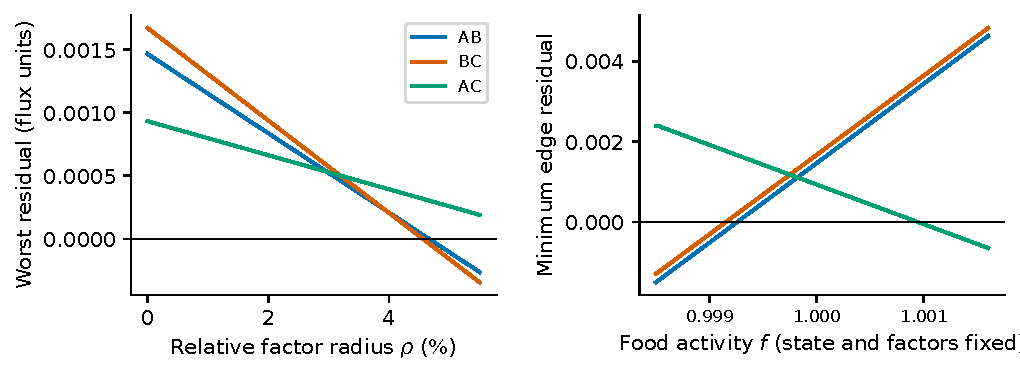
\includegraphics[width=\linewidth]{figures/operating.pdf}
\caption{Two separate slices at the weighted state. Left: the exact affine lower envelopes of the residuals under independent relative factor uncertainty, food fixed at one; the first zero is at $\rho_*=43/943$. Right: the edgewise minimum residual as the food activity varies with state and factors fixed; the window is~\eqref{eq:examplefood}. Neither panel is the joint certificate~\eqref{eq:jointmargin}.}
\label{fig:operating}
\end{figure}

\section{Formal verification}\label{sec:formal}

The statements marked as compiled in Table~\ref{tab:concordance} are Lean~4 theorems \citep{demoura2021} in the namespace \lean{ThermoCoreCompatibility.MultiInterface}, checked against Mathlib \citep{mathlib2020} with toolchain \lean{leanprover/lean4:v4.30.0} and a frozen dependency manifest. Verification promotes every warning to an error, rejects \lean{sorry}, probes the requested declarations, records the axioms each depends on, and hashes the sources. Every verified declaration depends only on \lean{propext}, \lean{Classical.choice} and \lean{Quot.sound}. Two receipts are kept: the root receipt for the source equivalence (module \lean{Root.lean}, source SHA-256 \lean{99270f83}\ldots, dependency manifest \lean{a8df0b60}\ldots, 67 seconds), and the extended receipt for the certificate lemmas and examples (module \lean{PostproofRoot.lean}, source SHA-256 \lean{c0f3b02a}\ldots, 102 seconds), whose dependency closure includes the unchanged root.

\paragraph{Architecture.} The development comprises about $1{,}000$ lines in 17 files and builds on the reversible-network semantics of \citep{tcic2026} and the pair-assembly source adapter of \citep{tcch2026}.
\begin{itemize}[before=\sloppy]
\item \lean{WeightedPair.lean}: the structure \lean{Factors} of positive $(a,b)$, the responses, the identity \lean{Factors.productive_iff} (Lemma~\ref{lem:edge}), strict monotonicity, the gap formula, $x^2<G<F<x$, and continuity.
\item \lean{PathResponse.lean}, \lean{PathReconstruction.lean}, \lean{PathCoordinates.lean}, \lean{PathEdges.lean}: the inductive \lean{Path} built by appending edges in physical order, the composed responses, the realization predicate, the interpolation orbit, the intermediate-value construction \lean{Path.sufficient}, and the boxed equivalence \lean{Path.boxed_iff} (Theorem~\ref{thm:path}); explicit vertex and edge coordinates for a path.
\item \lean{JunctionAssembly.lean}: the structure recording paths, vertex placement, the junction predicate, the endpoint characterization and private uniqueness; the merge lemma \lean{JunctionAssembly.merge} and the abstract equivalence \lean{compatible_iff_feasible}.
\item \lean{WeightedSource.lean}, \lean{JunctionSource.lean}: the weighted reversible network on the literal channels~\eqref{eq:chemistry} with per-channel barrier factors, the rebasing of each core motif with preserved PAC status, the identification of source-level productivity with \lean{Factors.Productive} (\lean{current_productive_iff}), the simple-graph structure \lean{SourceAssembly}, and the theorem \lean{sourceCompatible_iff_junctionFeasible} (Theorem~\ref{thm:main}).
\item \lean{RationalWitness.lean}, \lean{Examples.lean}, \lean{PostproofExamples.lean}: the decidable rational checker \lean{rationalFamilyCheck} and its soundness theorem at source level, the weighted example~\eqref{eq:witness} (\lean{Examples.weighted_source}), its unit-factor incompatibility, the four/five assembly (\lean{PostproofExamples.unit_source}), both nongradedness proofs, and exact evaluations of the radii, the $4\%$ residual bound and all 24 joint corners.
\item The four certificate modules \lean{RelativeRobustness.lean}, \lean{OperatingBox.lean}, \lean{FoodWindow.lean} and \lean{LinearCertificate.lean}: Propositions~\ref{prop:relative} and~\ref{prop:corner} (activity/food monotonicity and affine factor corners), the food window~\eqref{eq:foodwindow}, the scaling~\eqref{eq:scaling}, the instantaneous-loss equivalence~\eqref{eq:dilution}, and the deficit identities~\eqref{eq:deficit} with Proposition~\ref{prop:linear}.
\end{itemize}

\begin{table}[t]
\centering\small
\begin{tabular}{@{}>{\raggedright\arraybackslash}p{.30\linewidth}>{\raggedright\arraybackslash}p{.44\linewidth}>{\raggedright\arraybackslash}p{.19\linewidth}@{}}\toprule
Statement & Declaration or proof location & Evidence \\\midrule
One-edge interval, Lemma~\ref{lem:edge} & \lean{Factors.productive_iff}, \lean{Factors.gap}, \lean{Factors.lower_strictMono} & Lean \\
Path reconstruction, Theorem~\ref{thm:path} & \lean{Path.realizes_iff}, \lean{Path.boxed_iff} & Lean \\
Merge and assembly, Theorem~\ref{thm:main} & \lean{JunctionAssembly.merge}, \lean{sourceCompatible_iff_junctionFeasible} & Lean \\
Obstructions, Proposition~\ref{prop:obstructions} & \lean{Factors.decreases}; \lean{Examples.unit_source_incompatible} & Lean \\
Rational checker & \lean{rationalFamilyCheck_sound} & Lean \\
Representation, Lemma~\ref{lem:representation} & Section~\ref{sec:algorithm}; recurrence pilot & Conventional \\
Slack, precision, bisection, Lemmas~\ref{lem:slack}--\ref{lem:bisection} & Section~\ref{sec:algorithm}; backend \citep[Thm.\ 2.27]{basu2014} & Conventional \\
Bit bound, Theorem~\ref{thm:algorithm} & Section~\ref{sec:algorithm} & Conventional \\
Finite deficit, Proposition~\ref{prop:linear} & \lean{deficit_identities}, \lean{deficit_productive}, \lean{deficit_box} & Lean \\
LP complexity & Section~\ref{sec:linear}, \citep{khachiyan1979} & Conventional \\
Four/five assembly, nongraded & \lean{PostproofExamples.unit_source}, \lean{PostproofExamples.nongraded} & Lean \\
Relative radius, Proposition~\ref{prop:relative} & \lean{relative_box_iff}, \lean{relative_radius_iff} & Lean \\
Eight corners, Proposition~\ref{prop:corner} & \lean{activity_corner}, \lean{factor_corners}; composition in the proof & Lean lemmas \\
Food, scaling, loss & \lean{food_window}, \lean{food_scaling}, \lean{instantaneous_loss} & Lean \\
Printed operating numbers & \lean{PostproofExamples.weighted_relative}, \lean{joint_corner_values}; exact replay script & Lean and exact replay \\\bottomrule
\end{tabular}
\caption{Theorem/evidence concordance. Lean names are relative to the namespace of the development.}
\label{tab:concordance}
\end{table}

\paragraph{Boundary.} Three things are conventional and are not claimed to be verified: the instantiation of the external quantifier-elimination bound, the bit-size accounting of Section~\ref{sec:algorithm}, and the polynomial complexity of rational linear programming. The executable demonstration of Section~\ref{sec:demo} is not a verified program, and its Python validator and data encoder are trusted only through the checking argument of Step~1; a supplied \textsc{sat} state, however, is validated by the compiled soundness theorem of the rational checker once its data are transcribed. Every rational number printed in Sections~\ref{sec:linear} and~\ref{sec:operating} is replayed by a standard-library script distributed with the source.

\section{Discussion}\label{sec:discussion}

\paragraph{What the reduction shows.} Compatibility of a junction--path assembly is a property of its junction activities alone, and the property is explicit: two composed quadratic responses per path. Nothing about the interior is lost, because the interpolation orbit realizes every value strictly between the composed responses. This is stronger than a relaxation: the linear relaxations of \citep{tcic2026,tcch2026} discard the equation $y_{2X_u}=x_u^2$, whereas the path reduction keeps it and discards only variables that are provably recoverable.

\paragraph{The role of the factors.} The unit-factor shortcut is incompatible for every positive state, while factors $(9,1),(9,1),(2,1)$ admit a common state with all residuals positive and a $4.6\%$ independent factor tolerance. Since compatibility depends only on the ratios $a_e/b_e$, the picture is that of a response band per path whose width scales with $a_e b_e/((a_e+b_e)(a_e+2b_e))$; a shortcut with a slower first channel relative to its doubling channel has a lower band that can dip below the upper band of a longer path. Whether a given topology admits \emph{some} factor assignment making it compatible is a question on the closure of the union of the bands and is not addressed here.

\paragraph{Limits.} The decomposition is input; minimizing $k$ over decompositions, or recognizing whether an assembly with a small $k$ exists, is not treated. Private species share one box, and Remark~\ref{rem:privatebox} shows that independent private boxes break the two-function reduction. Cores are the two-reaction gain-two motif; higher gains and cores that share physical reactions are outside the class. The complexity bound is singly exponential in $k$ through the elimination routine and depends exponentially on $h$ through the expanded degree; neither dependence is shown to be necessary. The operating certificates quantify a fixed state; they do not assert that the state is reached, maintained or selected by any dynamics.

\paragraph{Open questions.}
\begin{enumerate}[label=(\arabic*)]
\item Is there a decision procedure for junction--path assemblies whose cost is polynomial in $h$, for instance by working with the recursive representation of $G_P,F_P$ instead of the expanded polynomial?
\item For which oriented simple graphs does some positive factor assignment make the whole edge family compatible? Directed cycles never do; the shortcut does; a characterization is open.
\item Can arbitrary private boxes be handled by introducing at most one additional variable per boxed private species, and does the resulting exponent remain $O(k'+1)$ in the enlarged variable count $k'$?
\item Does a common productive state of a junction--path assembly persist under the mass-action dynamics with the food chemostatted and a dilution below \eqref{eq:dilution}, and if so on what time scale?
\end{enumerate}

\paragraph{Reproducibility.} The source of this paper, the bibliography, the figure generator, the exact replay script and the data it reads are distributed together; the Lean development, the verification receipts, the executable demonstration and the conventional proof notes are in the accompanying repository.

\bibliographystyle{unsrtnat}
\bibliography{refs}

\end{document}
